\documentclass[12pt,a4paper]{article}
\newcommand{\AuthorName}
{نام و نام خانوادگی}
\newcommand{\AuthorSTID}
{شماره دانشجویی}

\usepackage{commons/course}

\lstset{
numbers=left, 
numberstyle=\small, 
numbersep=8pt, 
frame = single, 
language=Python,
framexleftmargin=15pt
}





%
%\let\ds\displaystyle
%\usepackage{arabtex}
%\usepackage[utf8]{inputenc}
%\usepackage[LFE,LAE]{fontenc}
%\usepackage[english,farsi]{babel}
%

\definecolor{dkgreen}{rgb}{0,0.6,0}
\definecolor{gray}{rgb}{0.5,0.5,0.5}
\definecolor{mauve}{rgb}{0.58,0,0.82}

\lstset{frame=tb,
aboveskip=3mm,
belowskip=3mm,
showstringspaces=false,
columns=flexible,
basicstyle={\small\ttfamily},
%numbers=none,
numberstyle=\tiny\color{gray},
keywordstyle=\color{blue},
commentstyle=\color{dkgreen},
stringstyle=\color{mauve},
breaklines=true,
breakatwhitespace=true,
tabsize=3
}

\begin{document}



\سربرگ{تمرین سری اول}{اسکنر و گراف نحو}{99/7/22}




 اعضای گروه: آزاده نحوی(97243098)، نگار رضوانفر(97243104)

						
\مسئله{تشخیص comment}

\پاسخ{}

\begin{center}
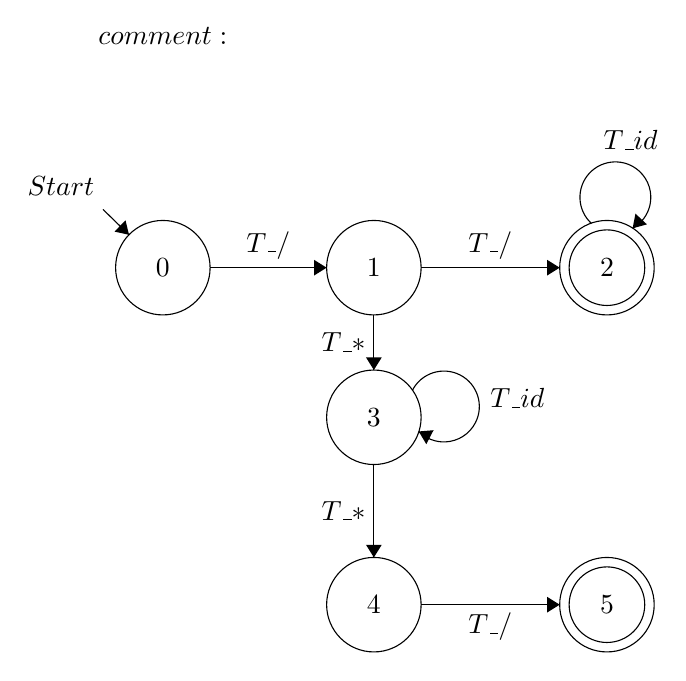
\begin{tikzpicture}[scale=0.2]
\tikzstyle{every node}+=[inner sep=0pt]
\draw [black] (9.8,-19.5) circle (3);
\draw (9.8,-19.5) node {$0$};
\draw [black] (23.2,-19.5) circle (3);
\draw (23.2,-19.5) node {$1$};
\draw [black] (23.2,-40.9) circle (3);
\draw (23.2,-40.9) node {$4$};
\draw [black] (38,-40.9) circle (3);
\draw (38,-40.9) node {$5$};
\draw [black] (38,-40.9) circle (2.4);
\draw [black] (38,-19.5) circle (3);
\draw (38,-19.5) node {$2$};
\draw [black] (38,-19.5) circle (2.4);
\draw [black] (23.2,-29) circle (3);
\draw (23.2,-29) node {$3$};
%\draw [black] (9.8,-4.8) circle (3);
\draw (9.8,-4.8) node {$comment:$};
\draw [black] (12.8,-19.5) -- (20.2,-19.5);
\fill [black] (20.2,-19.5) -- (19.4,-19) -- (19.4,-20);
\draw (16.5,-19) node [above] {$T\_/$};
\draw [black] (26.2,-19.5) -- (35,-19.5);
\fill [black] (35,-19.5) -- (34.2,-19) -- (34.2,-20);
\draw (30.6,-19) node [above] {$T\_/$};
\draw [black] (23.2,-22.5) -- (23.2,-26);
\fill [black] (23.2,-26) -- (23.7,-25.2) -- (22.7,-25.2);
\draw (22.7,-24.25) node [left] {$T\_*$};
\draw [black] (23.2,-32) -- (23.2,-37.9);
\fill [black] (23.2,-37.9) -- (23.7,-37.1) -- (22.7,-37.1);
\draw (22.7,-34.95) node [left] {$T\_*$};
\draw [black] (26.2,-40.9) -- (35,-40.9);
\fill [black] (35,-40.9) -- (34.2,-40.4) -- (34.2,-41.4);
\draw (30.6,-41.4) node [below] {$T\_/$};
\draw [black] (25.647,-27.285) arc (152.74616:-135.25384:2.25);
\draw (30.57,-27.78) node [right] {$T\_id$};
\fill [black] (26.05,-29.9) -- (26.53,-30.71) -- (26.99,-29.82);
\draw [black] (37.006,-16.682) arc (227.15723:-60.84277:2.25);
\draw (39.5,-12.06) node [above] {$T\_id$};
\fill [black] (39.63,-17) -- (40.54,-16.75) -- (39.81,-16.07);
\draw [black] (6,-15.8) -- (7.65,-17.41);
\draw (5.47,-14.33) node [left] {$Start$};
\fill [black] (7.65,-17.41) -- (7.43,-16.49) -- (6.73,-17.21);
\end{tikzpicture}
\end{center}



\pagebreak

\begin{center}
\LTR
\begin{lstlisting}

public class Qu1 {
    public static void main(String[] args) {
        Scanner sc = new Scanner (System.in);
        String str = sc.next();

        switch (str){
            case "//" :
                System.out.println("Single comment");
                break;
            case "/*" :
                String[] commands = new String[2];
                while (sc.hasNext()){
                    commands[0] = sc.next();
                    commands[1] = sc.next();
                    if( commands[0].equals("*")){
                        if (commands[1].equals("/"))
                             System.out.println("multi line comments");
                          
                        break;
                    }
                }
                break;
        }
    }
    
}
\end{lstlisting}
\end{center}

\pagebreak


%نام و نام خانوادگی:
%شماره دانشجویی: 
\مسئله{تشخیص ID}


\پاسخ{}



\begin{center}
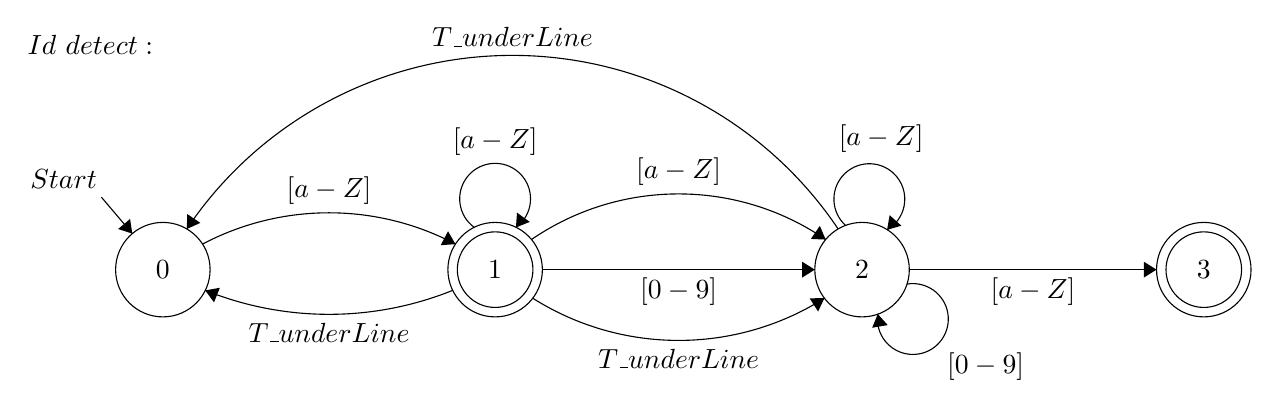
\begin{tikzpicture}[scale=0.2]
\tikzstyle{every node}+=[inner sep=0pt]
\draw [black] (10.1,-17.5) circle (3);
\draw (10.1,-17.5) node {$0$};
\draw [black] (54.5,-17.5) circle (3);
\draw (54.5,-17.5) node {$2$};
\draw [black] (76.2,-17.5) circle (3);
\draw (76.2,-17.5) node {$3$};
\draw [black] (76.2,-17.5) circle (2.4);
\draw [black] (31.2,-17.5) circle (3);
\draw (31.2,-17.5) node {$1$};
\draw [black] (31.2,-17.5) circle (2.4);
%\draw [black] (5.5,-3.2) circle (3);
\draw (5.5,-3.2) node {$Id\mbox{ }detect:$};
\draw [black] (6.2,-12.9) -- (8.16,-15.21);
\draw (3.8,-12.41) node [above] {$Start$};
\fill [black] (8.16,-15.21) -- (8.02,-14.28) -- (7.26,-14.92);
\draw [black] (53.46,-14.698) arc (228.09386:-59.90614:2.25);
\draw (55.71,-10.07) node [above] {$[a-Z]$};
\fill [black] (56.09,-14.97) -- (57,-14.71) -- (56.25,-14.04);
\draw [black] (57.343,-18.419) arc (99.81585:-188.18415:2.25);
\draw (59.87,-23.68) node [right] {$[0-9]$};
\fill [black] (55.5,-20.32) -- (55.14,-21.19) -- (56.13,-21.02);
\draw [black] (12.619,-15.877) arc (117.80321:62.19679:17.219);
\fill [black] (28.68,-15.88) -- (28.21,-15.06) -- (27.74,-15.95);
\draw (20.65,-13.39) node [above] {$[a-Z]$};
\draw [black] (29.877,-14.82) arc (234:-54:2.25);
\draw (31.2,-10.25) node [above] {$[a-Z]$};
\fill [black] (32.52,-14.82) -- (33.4,-14.47) -- (32.59,-13.88);
\draw [black] (28.507,-18.815) arc (-68.05692:-111.94308:21.025);
\fill [black] (12.79,-18.82) -- (13.35,-19.58) -- (13.72,-18.65);
\draw (20.65,-20.84) node [below] {$T\_underLine$};
\draw [black] (33.506,-15.588) arc (124.45654:55.54346:16.515);
\fill [black] (52.19,-15.59) -- (51.82,-14.72) -- (51.25,-15.55);
\draw (42.85,-12.19) node [above] {$[a-Z]$};
\draw [black] (52.115,-19.313) arc (-57.71215:-122.28785:17.344);
\fill [black] (52.11,-19.31) -- (51.17,-19.32) -- (51.71,-20.16);
\draw (42.85,-22.5) node [below] {$T\_underLine$};
\draw [black] (34.2,-17.5) -- (51.5,-17.5);
\fill [black] (51.5,-17.5) -- (50.7,-17) -- (50.7,-18);
\draw (42.85,-18) node [below] {$[0-9]$};
\draw [black] (57.5,-17.5) -- (73.2,-17.5);
\fill [black] (73.2,-17.5) -- (72.4,-17) -- (72.4,-18);
\draw (65.35,-18) node [below] {$[a-Z]$};
\draw [black] (11.619,-14.915) arc (146.10588:33.89412:24.915);
\fill [black] (11.62,-14.92) -- (12.48,-14.53) -- (11.65,-13.97);
\draw (32.3,-3.39) node [above] {$T\_underLine$};
\end{tikzpicture}
\end{center}


\begin{center}
\LTR
\begin{lstlisting}

read(str);
if (str.charAt(0) in [a-z] or [A_Z]){
	int i=1;
	while(i < str.length() ){
		if(str.charAt(i) in [a-z] or [A_Z] or [0-9])
			i++;
		else if (str.charAt(i) == '-')
			if(str.charAt(i++)=='-')
				sout("No");
		else
			i++;
	}
}
if(str.length > 1)
	if(str.charAt(str.length) in [a-z] or [A_Z])
		sout("Yes");
	else
		sout("No");
\end{lstlisting}
\end{center}

\pagebreak

%نام و نام خانوادگی:
%شماره دانشجویی: 
\مسئله{تشخیص String}


\پاسخ{}

\begin{center}
\begin{tikzpicture}[scale=0.2]
\tikzstyle{every node}+=[inner sep=0pt]
%\draw [black] (7.3,-5.6) circle (3);
\draw (7.3,-5.6) node {$Double\mbox{ }Quotes:$};
\draw [black] (13.2,-15.2) circle (3);
\draw (13.2,-15.2) node {$0$};
\draw [black] (28.3,-15.2) circle (3);
\draw (28.3,-15.2) node {$1$};
\draw [black] (45.4,-15.2) circle (3);
\draw (45.4,-15.2) node {$2$};
\draw [black] (45.4,-15.2) circle (2.4);
\draw [black] (28.3,-31.8) circle (3);
\draw (28.3,-31.8) node {$3$};
\draw [black] (45.4,-31.8) circle (3);
\draw (45.4,-31.8) node {$4$};
\draw [black] (4.6,-15.2) -- (10.2,-15.2);
\draw (4.1,-15.2) node [left] {$start$};
\fill [black] (10.2,-15.2) -- (9.4,-14.7) -- (9.4,-15.7);
\draw [black] (16.2,-15.2) -- (25.3,-15.2);
\fill [black] (25.3,-15.2) -- (24.5,-14.7) -- (24.5,-15.7);
\draw (20.75,-15.7) node [below] {$T\_"$};
\draw [black] (26.977,-12.52) arc (234:-54:2.25);
\draw (28.3,-7.95) node [above] {$\Sigma-{T\_"}$};
\fill [black] (29.62,-12.52) -- (30.5,-12.17) -- (29.69,-11.58);
\draw [black] (31.3,-15.2) -- (42.4,-15.2);
\fill [black] (42.4,-15.2) -- (41.6,-14.7) -- (41.6,-15.7);
\draw (36.85,-15.7) node [below] {$T\_"$};
\draw [black] (28.3,-18.2) -- (28.3,-28.8);
\fill [black] (28.3,-28.8) -- (28.8,-28) -- (27.8,-28);
\draw (27.8,-23.5) node [left] {$T\_/$};
\draw [black] (31.3,-31.8) -- (42.4,-31.8);
\fill [black] (42.4,-31.8) -- (41.6,-31.3) -- (41.6,-32.3);
\draw (36.85,-32.3) node [below] {$T\_"$};
\draw [black] (26.841,-34.408) arc (-1.4933:-289.4933:2.25);
\draw (22.14,-36.98) node [left] {$T\_/$};
\fill [black] (25.34,-32.23) -- (24.56,-31.71) -- (24.53,-32.71);
\draw [black] (48.08,-30.477) arc (144:-144:2.25);
\draw (52.65,-31.8) node [right] {$\Sigma-{T\_"}$};
\fill [black] (48.08,-33.12) -- (48.43,-34) -- (49.02,-33.19);
\draw [black] (45.4,-28.8) -- (45.4,-18.2);
\fill [black] (45.4,-18.2) -- (44.9,-19) -- (45.9,-19);
\draw (45.9,-23.5) node [right] {$T\_"$};
\end{tikzpicture}
\end{center}








\begin{center}
\LTR
\begin{lstlisting}

int i = 1;
if(str.charAt(0) == ' " '){
	while(i<str.lenght()-1){
		if (str.charAt(i) in sigma - ' " ')
			i++;
		else if (str.charAt(i--) == '\')
			i += 2;

     }
}

if (str.charAt(str.lenght-1) == ' " ')
	sout("Yes");

\end{lstlisting}
\end{center}

\pagebreak


%نام و نام خانوادگی:
%شماره دانشجویی: 
\مسئله{اعداد اعشاری}

\پاسخ{}

\begin{center}
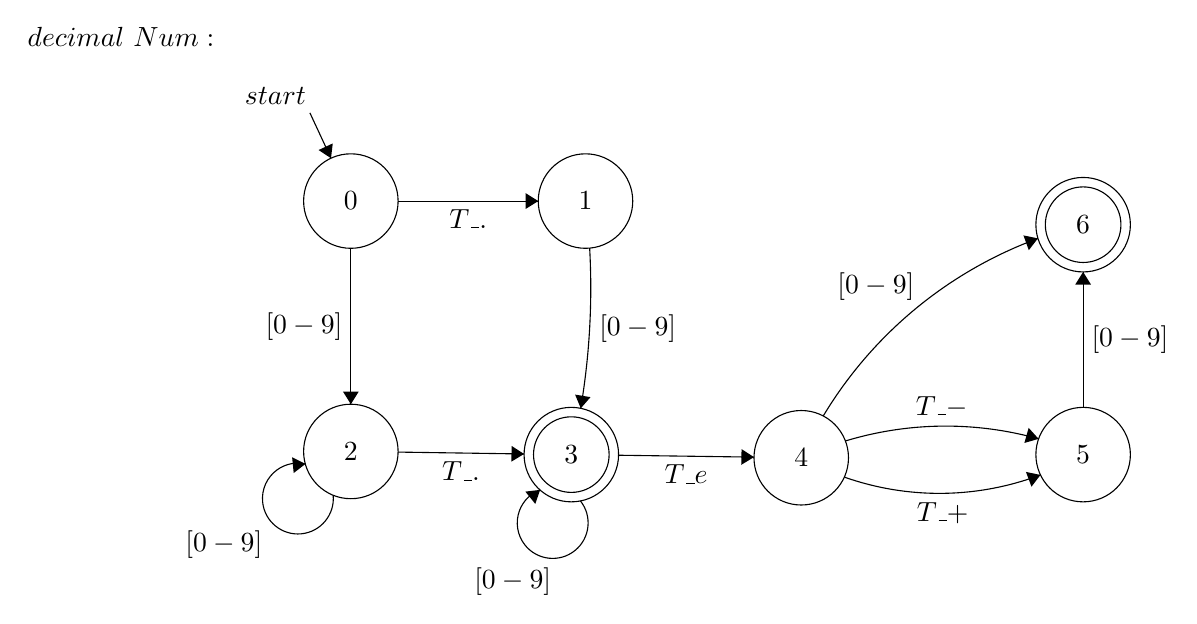
\begin{tikzpicture}[scale=0.2]
\tikzstyle{every node}+=[inner sep=0pt]
\draw [black] (22.1,-15.1) circle (3);
\draw (22.1,-15.1) node {$0$};
\draw [black] (37,-15.1) circle (3);
\draw (37,-15.1) node {$1$};
\draw [black] (22.1,-31) circle (3);
\draw (22.1,-31) node {$2$};
\draw [black] (36.1,-31.2) circle (3);
\draw (36.1,-31.2) node {$3$};
\draw [black] (36.1,-31.2) circle (2.4);
\draw [black] (50.7,-31.4) circle (3);
\draw (50.7,-31.4) node {$4$};
\draw [black] (68.6,-31.2) circle (3);
\draw (68.6,-31.2) node {$5$};
\draw [black] (68.6,-16.6) circle (3);
\draw (68.6,-16.6) node {$6$};
\draw [black] (68.6,-16.6) circle (2.4);
%\draw [black] (7.5,-4.7) circle (3);
\draw (7.5,-4.7) node {$decimal\mbox{ }Num:$};
\draw [black] (19.5,-9.5) -- (20.84,-12.38);
\draw (17.31,-8.98) node [above] {$start$};
\fill [black] (20.84,-12.38) -- (20.95,-11.44) -- (20.05,-11.86);
\draw [black] (25.1,-15.1) -- (34,-15.1);
\fill [black] (34,-15.1) -- (33.2,-14.6) -- (33.2,-15.6);
\draw (29.55,-15.6) node [below] {$T\_.$};
\draw [black] (22.1,-18.1) -- (22.1,-28);
\fill [black] (22.1,-28) -- (22.6,-27.2) -- (21.6,-27.2);
\draw (21.6,-23.05) node [left] {$[0-9]$};
\draw [black] (25.1,-31.04) -- (33.1,-31.16);
\fill [black] (33.1,-31.16) -- (32.31,-30.65) -- (32.29,-31.65);
\draw (29.09,-31.63) node [below] {$T\_.$};
\draw [black] (39.1,-31.24) -- (47.7,-31.36);
\fill [black] (47.7,-31.36) -- (46.91,-30.85) -- (46.89,-31.85);
\draw (43.39,-31.83) node [below] {$T\_e$};
\draw [black] (65.894,-32.488) arc (-69.27811:-109.44159:18.146);
\fill [black] (65.89,-32.49) -- (64.97,-32.3) -- (65.32,-33.24);
\draw (59.68,-34.19) node [below] {$T\_+$};
\draw [black] (53.502,-30.335) arc (106.89197:74.38832:21.928);
\fill [black] (65.77,-30.2) -- (65.14,-29.5) -- (64.87,-30.46);
\draw (59.62,-28.87) node [above] {$T\_-$};
\draw [black] (20.976,-33.769) arc (5.63354:-282.36646:2.25);
\draw (16.51,-36.94) node [left] {$[0-9]$};
\fill [black] (19.22,-31.79) -- (18.37,-31.37) -- (18.47,-32.37);
\draw [black] (36.671,-34.133) arc (38.74488:-249.25512:2.25);
\draw (32.38,-38.36) node [below] {$[0-9]$};
\fill [black] (34.12,-33.44) -- (33.18,-33.55) -- (33.81,-34.33);
\draw [black] (68.6,-28.2) -- (68.6,-19.6);
\fill [black] (68.6,-19.6) -- (68.1,-20.4) -- (69.1,-20.4);
\draw (69.1,-23.9) node [right] {$[0-9]$};
\draw [black] (52.097,-28.747) arc (148.9937:110.17525:26.618);
\fill [black] (65.73,-17.47) -- (64.81,-17.28) -- (65.15,-18.22);
\draw (55.44,-21.45) node [above] {$[0-9]$};
\draw [black] (37.264,-18.088) arc (3.17349:-9.57256:45.892);
\fill [black] (36.7,-28.26) -- (37.32,-27.55) -- (36.34,-27.39);
\draw (37.84,-23.22) node [right] {$[0-9]$};
\end{tikzpicture}
\end{center}


\pagebreak

%نام و نام خانوادگی:
%شماره دانشجویی: 
\مسئله{تشخیص عبارت های ریاضی}

\پاسخ{}\begin{center}
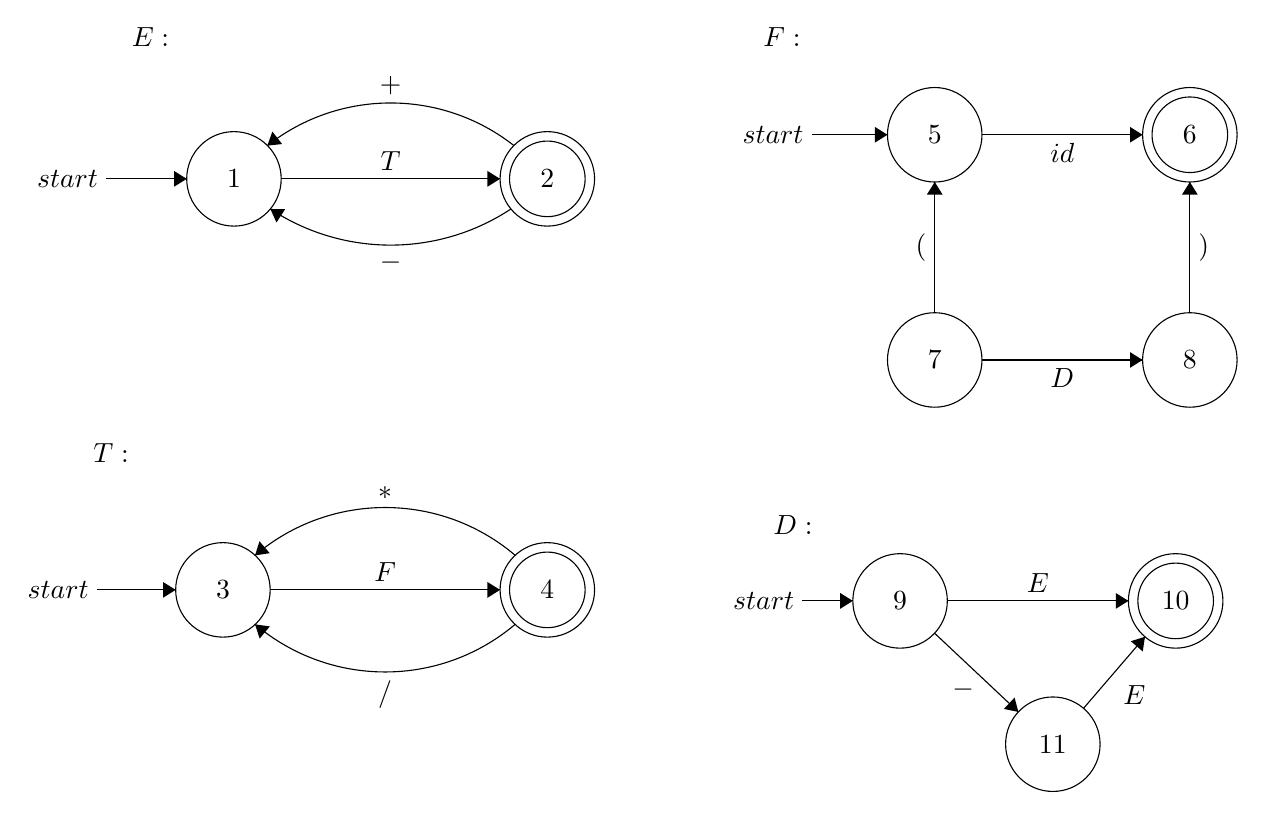
\begin{tikzpicture}[scale=0.2]
\tikzstyle{every node}+=[inner sep=0pt]
%\draw [black] (8.6,-8.6) circle (3);
\draw (8.6,-8.6) node {$E:$};
\draw [black] (13.9,-17.6) circle (3);
\draw (13.9,-17.6) node {$1$};
\draw [black] (33.8,-17.6) circle (3);
\draw (33.8,-17.6) node {$2$};
\draw [black] (33.8,-17.6) circle (2.4);
%\draw [black] (6.1,-35) circle (3);
\draw (6.1,-35) node {$T:$};
\draw [black] (13.2,-43.7) circle (3);
\draw (13.2,-43.7) node {$3$};
\draw [black] (33.8,-43.7) circle (3);
\draw (33.8,-43.7) node {$4$};
\draw [black] (33.8,-43.7) circle (2.4);
%\draw [black] (48.7,-8.6) circle (3);
\draw (48.7,-8.6) node {$F:$};
\draw [black] (58.4,-14.8) circle (3);
\draw (58.4,-14.8) node {$5$};
\draw [black] (74.6,-14.8) circle (3);
\draw (74.6,-14.8) node {$6$};
\draw [black] (74.6,-14.8) circle (2.4);
\draw [black] (58.4,-29.1) circle (3);
\draw (58.4,-29.1) node {$7$};
\draw [black] (74.6,-29.1) circle (3);
\draw (74.6,-29.1) node {$8$};
%\draw [black] (49.4,-39.6) circle (3);
\draw (49.4,-39.6) node {$D:$};
\draw [black] (56.2,-44.4) circle (3);
\draw (56.2,-44.4) node {$9$};
\draw [black] (73.7,-44.4) circle (3);
\draw (73.7,-44.4) node {$10$};
\draw [black] (73.7,-44.4) circle (2.4);
\draw [black] (65.9,-53.5) circle (3);
\draw (65.9,-53.5) node {$11$};
\draw [black] (5.8,-17.6) -- (10.9,-17.6);
\draw (5.3,-17.6) node [left] {$start$};
\fill [black] (10.9,-17.6) -- (10.1,-17.1) -- (10.1,-18.1);
\draw [black] (16.02,-15.487) arc (128.13473:51.86527:12.681);
\fill [black] (16.02,-15.49) -- (16.96,-15.39) -- (16.34,-14.6);
\draw (23.85,-12.28) node [above] {$+$};
\draw [black] (31.494,-19.51) arc (-56.55185:-123.44815:13.869);
\fill [black] (16.21,-19.51) -- (16.6,-20.37) -- (17.15,-19.53);
\draw (23.85,-22.31) node [below] {$-$};
\draw [black] (16.9,-17.6) -- (30.8,-17.6);
\fill [black] (30.8,-17.6) -- (30,-17.1) -- (30,-18.1);
\draw (23.85,-17.1) node [above] {$T$};
\draw [black] (15.237,-41.507) arc (130.36754:49.63246:12.757);
\fill [black] (15.24,-41.51) -- (16.17,-41.37) -- (15.52,-40.61);
\draw (23.5,-37.97) node [above] {$*$};
\draw [black] (31.757,-45.888) arc (-49.76228:-130.23772:12.783);
\fill [black] (15.24,-45.89) -- (15.53,-46.79) -- (16.18,-46.02);
\draw (23.5,-49.41) node [below] {$/$};
\draw [black] (16.2,-43.7) -- (30.8,-43.7);
\fill [black] (30.8,-43.7) -- (30,-43.2) -- (30,-44.2);
\draw (23.5,-43.2) node [above] {$F$};
\draw [black] (5.2,-43.7) -- (10.2,-43.7);
\draw (4.7,-43.7) node [left] {$start$};
\fill [black] (10.2,-43.7) -- (9.4,-43.2) -- (9.4,-44.2);
\draw [black] (50.6,-14.8) -- (55.4,-14.8);
\draw (50.1,-14.8) node [left] {$start$};
\fill [black] (55.4,-14.8) -- (54.6,-14.3) -- (54.6,-15.3);
\draw [black] (61.4,-14.8) -- (71.6,-14.8);
\fill [black] (71.6,-14.8) -- (70.8,-14.3) -- (70.8,-15.3);
\draw (66.5,-15.3) node [below] {$id$};
\draw [black] (74.6,-26.1) -- (74.6,-17.8);
\fill [black] (74.6,-17.8) -- (74.1,-18.6) -- (75.1,-18.6);
\draw (75.1,-21.95) node [right] {$)$};
\draw [black] (58.4,-26.1) -- (58.4,-17.8);
\fill [black] (58.4,-17.8) -- (57.9,-18.6) -- (58.9,-18.6);
\draw (57.9,-21.95) node [left] {$($};
\draw [black] (61.4,-29.1) -- (71.6,-29.1);
\fill [black] (71.6,-29.1) -- (70.8,-28.6) -- (70.8,-29.6);
\draw (66.5,-29.6) node [below] {$D$};
\draw [black] (59.2,-44.4) -- (70.7,-44.4);
\fill [black] (70.7,-44.4) -- (69.9,-43.9) -- (69.9,-44.9);
\draw (64.95,-43.9) node [above] {$E$};
\draw [black] (67.85,-51.22) -- (71.75,-46.68);
\fill [black] (71.75,-46.68) -- (70.85,-46.96) -- (71.61,-47.61);
\draw (70.35,-50.39) node [right] {$E$};
\draw [black] (58.39,-46.45) -- (63.71,-51.45);
\fill [black] (63.71,-51.45) -- (63.47,-50.54) -- (62.79,-51.26);
\draw (60.2,-49.43) node [below] {$-$};
\draw [black] (50,-44.4) -- (53.2,-44.4);
\draw (49.5,-44.4) node [left] {$start$};
\fill [black] (53.2,-44.4) -- (52.4,-43.9) -- (52.4,-44.9);
\end{tikzpicture}
\end{center}

%نام و نام خانوادگی:
%شماره دانشجویی: 
\مسئله{تشخیص بولین}

\پاسخ{}

\begin{center}
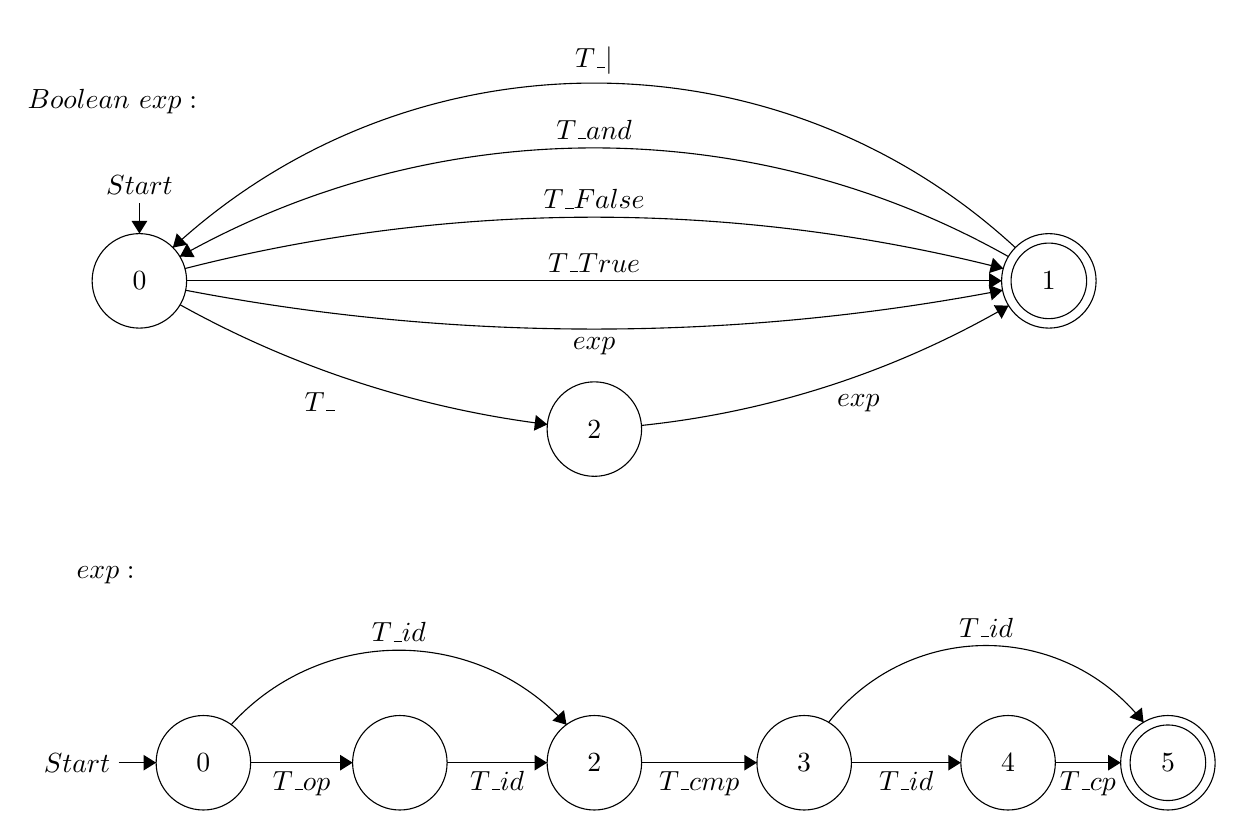
\begin{tikzpicture}[scale=0.2]
\tikzstyle{every node}+=[inner sep=0pt]
\draw [black] (9.316,-15.744) circle (3);
\draw (9.32,-15.74) node {$0$};
\draw [black] (67.068,-15.744) circle (3);
\draw (67.07,-15.74) node {$1$};
\draw [black] (67.068,-15.744) circle (2.4);
\draw [black] (38.208,-25.156) circle (3);
\draw (38.21,-25.16) node {$2$};
%\draw [black] (7.6,-4.384) circle (3);
\draw (7.6,-4.38) node {$Boolean\mbox{ }exp:$};
\draw [black] (13.38,-46.344) circle (3);
\draw (13.38,-46.34) node {$0$};
\draw [black] (38.208,-46.344) circle (3);
\draw (38.21,-46.34) node {$2$};
\draw [black] (51.532,-46.344) circle (3);
\draw (51.53,-46.34) node {$3$};
\draw [black] (64.48,-46.344) circle (3);
\draw (64.48,-46.34) node {$4$};
\draw [black] (74.628,-46.344) circle (3);
\draw (74.63,-46.34) node {$5$};
\draw [black] (74.628,-46.344) circle (2.4);
\draw [black] (25.856,-46.344) circle (3);
%\draw [black] (7.168,-34.448) circle (3);
\draw (7.17,-34.45) node {$exp:$};
\draw [black] (9.32,-10.8) -- (9.32,-12.74);
\draw (9.32,-10.3) node [above] {$Start$};
\fill [black] (9.32,-12.74) -- (9.82,-11.94) -- (8.82,-11.94);
\draw [black] (35.223,-24.859) arc (-97.02999:-119.05759:64.189);
\fill [black] (35.22,-24.86) -- (34.49,-24.26) -- (34.37,-25.26);
\draw (21.06,-22.78) node [below] {$T\_~$};
\draw [black] (64.515,-17.319) arc (-59.81134:-84.06365:58.374);
\fill [black] (64.51,-17.32) -- (63.57,-17.29) -- (64.07,-18.15);
\draw (54.97,-22.93) node [below] {$exp$};
\draw [black] (64.128,-16.341) arc (-79.13814:-100.86186:137.635);
\fill [black] (64.13,-16.34) -- (63.25,-16) -- (63.44,-16.98);
\draw (38.19,-19.31) node [below] {$exp$};
\draw [black] (12.32,-15.74) -- (64.07,-15.74);
\fill [black] (64.07,-15.74) -- (63.27,-15.24) -- (63.27,-16.24);
\draw (38.19,-15.24) node [above] {$T\_True$};
\draw [black] (12.212,-14.961) arc (104.31546:75.68454:105.072);
\fill [black] (64.17,-14.96) -- (63.52,-14.28) -- (63.27,-15.25);
\draw (38.19,-11.2) node [above] {$T\_False$};
\draw [black] (11.887,-14.199) arc (119.39832:60.60168:53.587);
\fill [black] (11.89,-14.2) -- (12.83,-14.24) -- (12.34,-13.37);
\draw (38.19,-6.8) node [above] {$T\_and$};
\draw [black] (11.443,-13.629) arc (132.66778:47.33222:39.468);
\fill [black] (11.44,-13.63) -- (12.37,-13.45) -- (11.69,-12.72);
\draw (38.19,-2.68) node [above] {$T\_|$};
\draw [black] (8,-46.34) -- (10.38,-46.34);
\draw (7.5,-46.34) node [left] {$Start$};
\fill [black] (10.38,-46.34) -- (9.58,-45.84) -- (9.58,-46.84);
\draw [black] (41.21,-46.34) -- (48.53,-46.34);
\fill [black] (48.53,-46.34) -- (47.73,-45.84) -- (47.73,-46.84);
\draw (44.87,-46.84) node [below] {$T\_cmp$};
\draw [black] (54.53,-46.34) -- (61.48,-46.34);
\fill [black] (61.48,-46.34) -- (60.68,-45.84) -- (60.68,-46.84);
\draw (58.01,-46.84) node [below] {$T\_id$};
\draw [black] (67.48,-46.34) -- (71.63,-46.34);
\fill [black] (71.63,-46.34) -- (70.83,-45.84) -- (70.83,-46.84);
\draw (69.55,-46.84) node [below] {$T\_cp$};
\draw [black] (15.146,-43.925) arc (137.8857:42.1143:14.355);
\fill [black] (36.44,-43.93) -- (36.28,-43) -- (35.54,-43.67);
\draw (25.79,-38.7) node [above] {$T\_id$};
\draw [black] (16.38,-46.34) -- (22.86,-46.34);
\fill [black] (22.86,-46.34) -- (22.06,-45.84) -- (22.06,-46.84);
\draw (19.62,-46.84) node [below] {$T\_op$};
\draw [black] (28.86,-46.34) -- (35.21,-46.34);
\fill [black] (35.21,-46.34) -- (34.41,-45.84) -- (34.41,-46.84);
\draw (32.03,-46.84) node [below] {$T\_id$};
\draw [black] (53.081,-43.783) arc (142.0598:37.9402:12.679);
\fill [black] (73.08,-43.78) -- (72.98,-42.84) -- (72.19,-43.46);
\draw (63.08,-38.4) node [above] {$T\_id$};
\end{tikzpicture}
\end{center}


\pagebreak

%نام و نام خانوادگی:
%شماره دانشجویی: 
\مسئله{else-if}

\پاسخ{}
\begin{center}
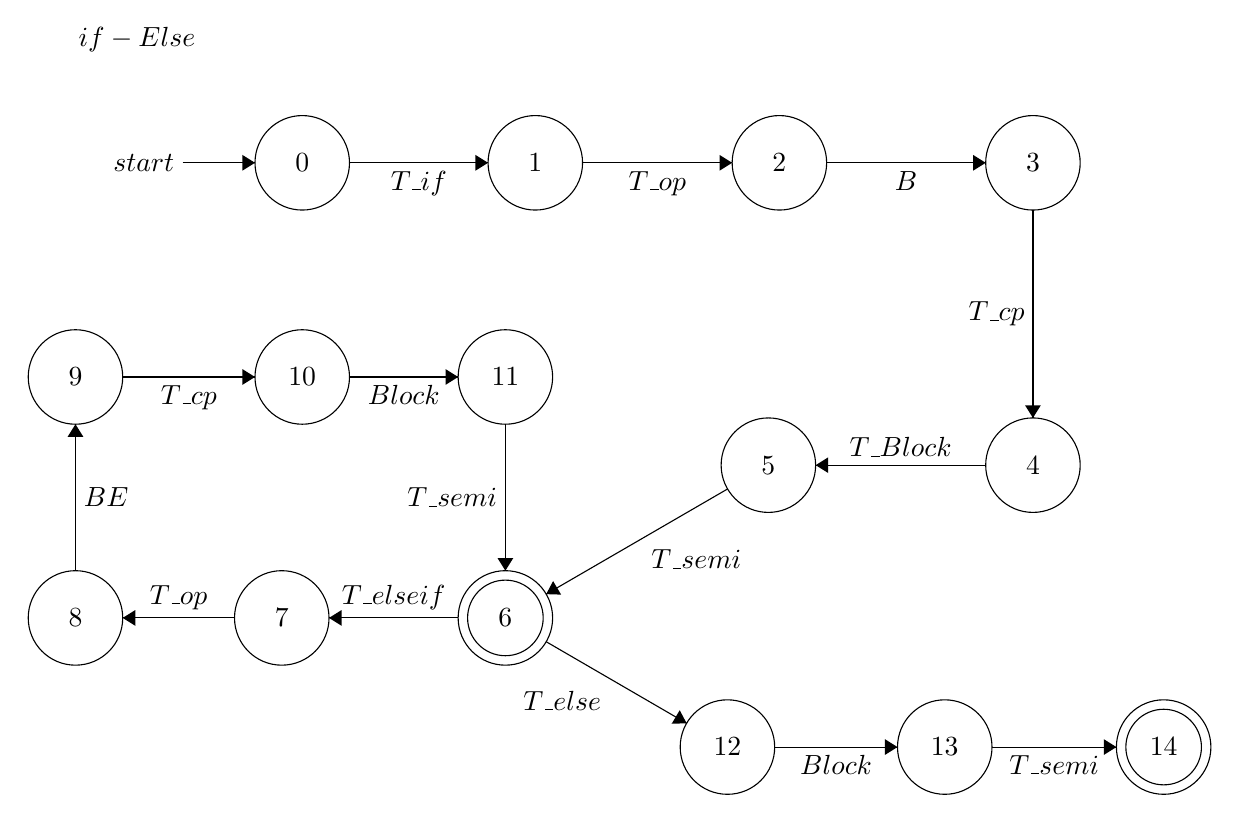
\begin{tikzpicture}[scale=0.2]
\tikzstyle{every node}+=[inner sep=0pt]

\draw (9.5,-6.9) node {$if-Else$};
\draw [black] (20,-14.7) circle (3);
\draw (20,-14.7) node {$0$};
\draw [black] (34.8,-14.7) circle (3);
\draw (34.8,-14.7) node {$1$};
\draw [black] (50.3,-14.7) circle (3);
\draw (50.3,-14.7) node {$2$};
\draw [black] (66.4,-14.7) circle (3);
\draw (66.4,-14.7) node {$3$};
\draw [black] (66.4,-33.9) circle (3);
\draw (66.4,-33.9) node {$4$};
\draw [black] (49.6,-33.9) circle (3);
\draw (49.6,-33.9) node {$5$};
\draw [black] (32.9,-43.6) circle (3);
\draw (32.9,-43.6) node {$6$};
\draw [black] (32.9,-43.6) circle (2.4);
\draw [black] (18.7,-43.6) circle (3);
\draw (18.7,-43.6) node {$7$};
\draw [black] (5.6,-43.6) circle (3);
\draw (5.6,-43.6) node {$8$};
\draw [black] (5.6,-28.3) circle (3);
\draw (5.6,-28.3) node {$9$};
\draw [black] (20,-28.3) circle (3);
\draw (20,-28.3) node {$10$};
\draw [black] (32.9,-28.3) circle (3);
\draw (32.9,-28.3) node {$11$};
\draw [black] (47,-51.8) circle (3);
\draw (47,-51.8) node {$12$};
\draw [black] (60.8,-51.8) circle (3);
\draw (60.8,-51.8) node {$13$};
\draw [black] (74.7,-51.8) circle (3);
\draw (74.7,-51.8) node {$14$};
\draw [black] (74.7,-51.8) circle (2.4);
\draw [black] (12.4,-14.7) -- (17,-14.7);
\draw (11.9,-14.7) node [left] {$start$};
\fill [black] (17,-14.7) -- (16.2,-14.2) -- (16.2,-15.2);
\draw [black] (23,-14.7) -- (31.8,-14.7);
\fill [black] (31.8,-14.7) -- (31,-14.2) -- (31,-15.2);
\draw (27.4,-15.2) node [below] {$T\_if$};
\draw [black] (37.8,-14.7) -- (47.3,-14.7);
\fill [black] (47.3,-14.7) -- (46.5,-14.2) -- (46.5,-15.2);
\draw (42.55,-15.2) node [below] {$T\_op$};
\draw [black] (53.3,-14.7) -- (63.4,-14.7);
\fill [black] (63.4,-14.7) -- (62.6,-14.2) -- (62.6,-15.2);
\draw (58.35,-15.2) node [below] {$B$};
\draw [black] (66.4,-17.7) -- (66.4,-30.9);
\fill [black] (66.4,-30.9) -- (66.9,-30.1) -- (65.9,-30.1);
\draw (65.9,-24.3) node [left] {$T\_cp$};
\draw [black] (63.4,-33.9) -- (52.6,-33.9);
\fill [black] (52.6,-33.9) -- (53.4,-34.4) -- (53.4,-33.4);
\draw (58,-33.4) node [above] {$T\_Block$};
\draw [black] (47.01,-35.41) -- (35.49,-42.09);
\fill [black] (35.49,-42.09) -- (36.44,-42.12) -- (35.93,-41.26);
\draw (45.02,-39.25) node [below] {$T\_semi$};
\draw [black] (29.9,-43.6) -- (21.7,-43.6);
\fill [black] (21.7,-43.6) -- (22.5,-44.1) -- (22.5,-43.1);
\draw (25.8,-43.1) node [above] {$T\_elseif$};
\draw [black] (15.7,-43.6) -- (8.6,-43.6);
\fill [black] (8.6,-43.6) -- (9.4,-44.1) -- (9.4,-43.1);
\draw (12.15,-43.1) node [above] {$T\_op$};
\draw [black] (5.6,-40.6) -- (5.6,-31.3);
\fill [black] (5.6,-31.3) -- (5.1,-32.1) -- (6.1,-32.1);
\draw (6.1,-35.95) node [right] {$BE$};
\draw [black] (8.6,-28.3) -- (17,-28.3);
\fill [black] (17,-28.3) -- (16.2,-27.8) -- (16.2,-28.8);
\draw (12.8,-28.8) node [below] {$T\_cp$};
\draw [black] (23,-28.3) -- (29.9,-28.3);
\fill [black] (29.9,-28.3) -- (29.1,-27.8) -- (29.1,-28.8);
\draw (26.45,-28.8) node [below] {$Block$};
\draw [black] (32.9,-31.3) -- (32.9,-40.6);
\fill [black] (32.9,-40.6) -- (33.4,-39.8) -- (32.4,-39.8);
\draw (32.4,-35.95) node [left] {$T\_semi$};
\draw [black] (35.49,-45.11) -- (44.41,-50.29);
\fill [black] (44.41,-50.29) -- (43.97,-49.46) -- (43.46,-50.32);
\draw (36.51,-48.2) node [below] {$T\_else$};
\draw [black] (50,-51.8) -- (57.8,-51.8);
\fill [black] (57.8,-51.8) -- (57,-51.3) -- (57,-52.3);
\draw (53.9,-52.3) node [below] {$Block$};
\draw [black] (63.8,-51.8) -- (71.7,-51.8);
\fill [black] (71.7,-51.8) -- (70.9,-51.3) -- (70.9,-52.3);
\draw (67.75,-52.3) node [below] {$T\_semi$};
\end{tikzpicture}
\end{center}

\pagebreak

%نام و نام خانوادگی:
%شماره دانشجویی: 
\مسئله{switch case}

\پاسخ{}

\begin{center}
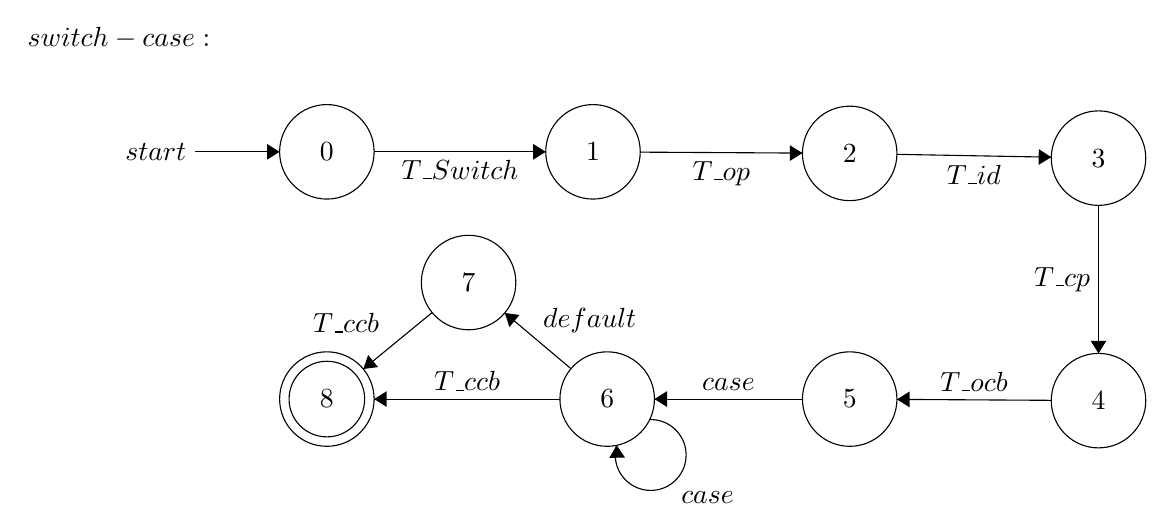
\begin{tikzpicture}[scale=0.2]
\tikzstyle{every node}+=[inner sep=0pt]
\draw (4.8,-20) node {$switch-case:$};
\draw [black] (18,-27.2) circle (3);
\draw (18,-27.2) node {$0$};
\draw [black] (34.9,-27.2) circle (3);
\draw (34.9,-27.2) node {$1$};
\draw [black] (51.2,-27.3) circle (3);
\draw (51.2,-27.3) node {$2$};
\draw [black] (67,-27.6) circle (3);
\draw (67,-27.6) node {$3$};
\draw [black] (67,-43) circle (3);
\draw (67,-43) node {$4$};
\draw [black] (51.2,-42.9) circle (3);
\draw (51.2,-42.9) node {$5$};
\draw [black] (35.8,-42.9) circle (3);
\draw (35.8,-42.9) node {$6$};
\draw [black] (27,-35.5) circle (3);
\draw (27,-35.5) node {$7$};
\draw [black] (18,-42.9) circle (3);
\draw (18,-42.9) node {$8$};
\draw [black] (18,-42.9) circle (2.4);
\draw [black] (21,-27.2) -- (31.9,-27.2);
\fill [black] (31.9,-27.2) -- (31.1,-26.7) -- (31.1,-27.7);
\draw (26.45,-27.7) node [below] {$T\_Switch$};
\draw [black] (37.9,-27.22) -- (48.2,-27.28);
\fill [black] (48.2,-27.28) -- (47.4,-26.78) -- (47.4,-27.78);
\draw (43.05,-27.77) node [below] {$T\_op$};
\draw [black] (54.2,-27.36) -- (64,-27.54);
\fill [black] (64,-27.54) -- (63.21,-27.03) -- (63.19,-28.03);
\draw (59.08,-28) node [below] {$T\_id$};
\draw [black] (67,-30.6) -- (67,-40);
\fill [black] (67,-40) -- (67.5,-39.2) -- (66.5,-39.2);
\draw (66.5,-35.3) node [left] {$T\_cp$};
\draw [black] (64,-42.98) -- (54.2,-42.92);
\fill [black] (54.2,-42.92) -- (55,-43.42) -- (55,-42.42);
\draw (59.1,-42.43) node [above] {$T\_ocb$};
\draw [black] (48.2,-42.9) -- (38.8,-42.9);
\fill [black] (38.8,-42.9) -- (39.6,-43.4) -- (39.6,-42.4);
\draw (43.5,-42.4) node [above] {$case$};
\draw [black] (38.489,-44.203) arc (91.87498:-196.12502:2.25);
\draw (42.17,-48.72) node [below] {$case$};
\fill [black] (36.4,-45.83) -- (35.93,-46.64) -- (36.93,-46.61);
\draw [black] (33.5,-40.97) -- (29.3,-37.43);
\fill [black] (29.3,-37.43) -- (29.59,-38.33) -- (30.23,-37.56);
\draw (34.69,-38.71) node [above] {$default$};
\draw [black] (32.8,-42.9) -- (21,-42.9);
\fill [black] (21,-42.9) -- (21.8,-43.4) -- (21.8,-42.4);
\draw (26.9,-42.4) node [above] {$T\_ccb$};
\draw [black] (24.68,-37.41) -- (20.32,-40.99);
\fill [black] (20.32,-40.99) -- (21.25,-40.87) -- (20.62,-40.1);
\draw (19.22,-38.71) node [above] {$T\_ccb$};
\draw [black] (9.6,-27.2) -- (15,-27.2);
\draw (9.1,-27.2) node [left] {$start$};
\fill [black] (15,-27.2) -- (14.2,-26.7) -- (14.2,-27.7);
\end{tikzpicture}
\end{center}






\begin{center}
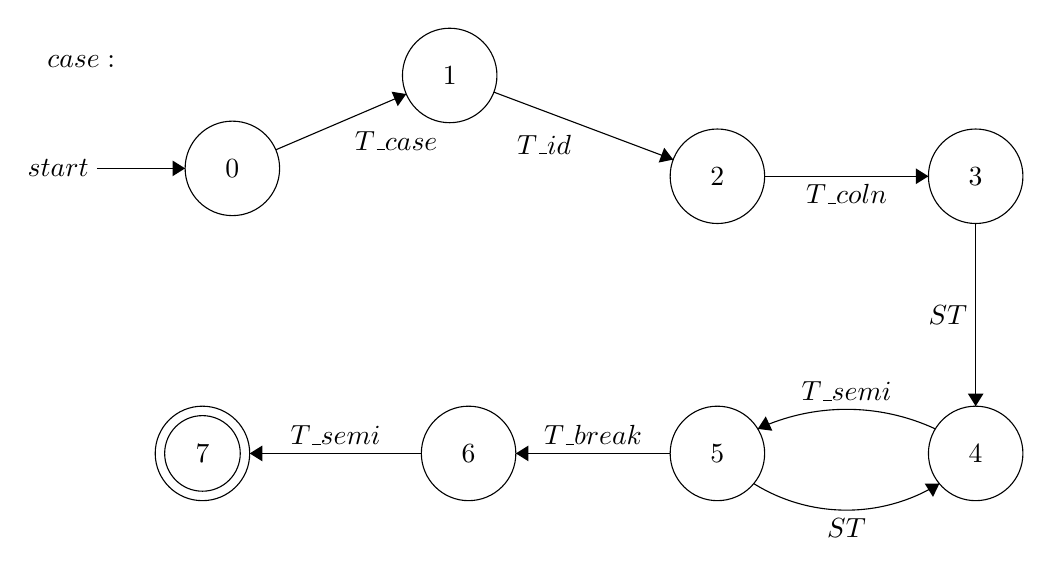
\begin{tikzpicture}[scale=0.2]
\tikzstyle{every node}+=[inner sep=0pt]
\draw [black] (14.4,-11.9) circle (3);
\draw (14.4,-11.9) node {$0$};
\draw [black] (28.2,-6) circle (3);
\draw (28.2,-6) node {$1$};
\draw [black] (45.2,-12.4) circle (3);
\draw (45.2,-12.4) node {$2$};
\draw [black] (61.6,-12.4) circle (3);
\draw (61.6,-12.4) node {$3$};
\draw [black] (61.6,-30) circle (3);
\draw (61.6,-30) node {$4$};
\draw [black] (45.2,-30) circle (3);
\draw (45.2,-30) node {$5$};
\draw [black] (29.4,-30) circle (3);
\draw (29.4,-30) node {$6$};
\draw [black] (12.5,-30) circle (3);
\draw (12.5,-30) node {$7$};
\draw [black] (12.5,-30) circle (2.4);

\draw (4.8,-5.1) node {$case:$};
\draw [black] (5.8,-11.9) -- (11.4,-11.9);
\draw (5.3,-11.9) node [left] {$start$};
\fill [black] (11.4,-11.9) -- (10.6,-11.4) -- (10.6,-12.4);
\draw [black] (17.16,-10.72) -- (25.44,-7.18);
\fill [black] (25.44,-7.18) -- (24.51,-7.03) -- (24.9,-7.95);
\draw (24.8,-9.5) node [below] {$T\_case$};
\draw [black] (31.01,-7.06) -- (42.39,-11.34);
\fill [black] (42.39,-11.34) -- (41.82,-10.59) -- (41.47,-11.53);
\draw (34.2,-9.76) node [below] {$T\_id$};
\draw [black] (48.2,-12.4) -- (58.6,-12.4);
\fill [black] (58.6,-12.4) -- (57.8,-11.9) -- (57.8,-12.9);
\draw (53.4,-12.9) node [below] {$T\_coln$};
\draw [black] (61.6,-15.4) -- (61.6,-27);
\fill [black] (61.6,-27) -- (62.1,-26.2) -- (61.1,-26.2);
\draw (61.1,-21.2) node [left] {$ST$};
\draw [black] (47.758,-28.444) arc (114.89901:65.10099:13.401);
\fill [black] (47.76,-28.44) -- (48.69,-28.56) -- (48.27,-27.65);
\draw (53.4,-26.7) node [above] {$T\_semi$};
\draw [black] (59.299,-31.911) arc (-58.01016:-121.98984:11.135);
\fill [black] (59.3,-31.91) -- (58.36,-31.91) -- (58.89,-32.76);
\draw (53.4,-34.1) node [below] {$ST$};
\draw [black] (42.2,-30) -- (32.4,-30);
\fill [black] (32.4,-30) -- (33.2,-30.5) -- (33.2,-29.5);
\draw (37.3,-29.5) node [above] {$T\_break$};
\draw [black] (26.4,-30) -- (15.5,-30);
\fill [black] (15.5,-30) -- (16.3,-30.5) -- (16.3,-29.5);
\draw (20.95,-29.5) node [above] {$T\_semi$};
\end{tikzpicture}
\end{center}





\begin{center}
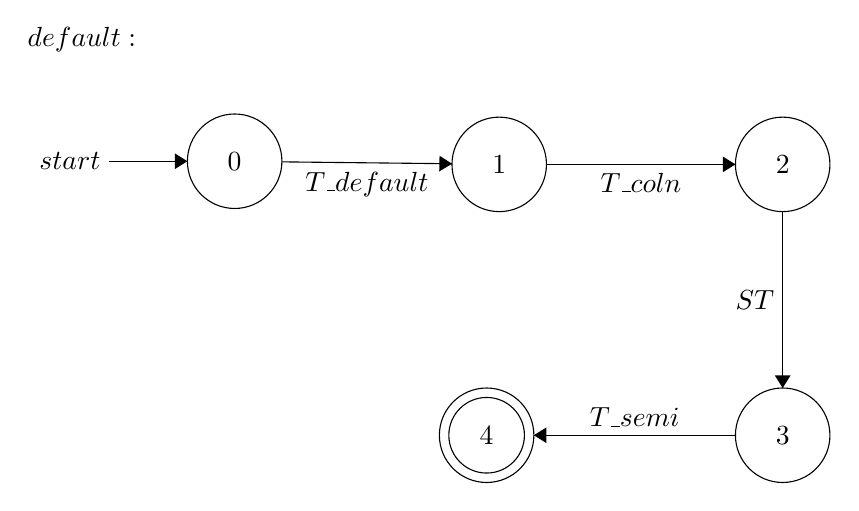
\begin{tikzpicture}[scale=0.2]
\tikzstyle{every node}+=[inner sep=0pt]
\draw [black] (19.2,-16.9) circle (3);
\draw (19.2,-16.9) node {$0$};
%\draw [black] (9.5,-9.2) circle (3);
\draw (9.5,-9.2) node {$default:$};
\draw [black] (36,-17.1) circle (3);
\draw (36,-17.1) node {$1$};
\draw [black] (54,-17.1) circle (3);
\draw (54,-17.1) node {$2$};
\draw [black] (54,-34.3) circle (3);
\draw (54,-34.3) node {$3$};
\draw [black] (35.2,-34.3) circle (3);
\draw (35.2,-34.3) node {$4$};
\draw [black] (35.2,-34.3) circle (2.4);
\draw [black] (11.2,-16.9) -- (16.2,-16.9);
\draw (10.7,-16.9) node [left] {$start$};
\fill [black] (16.2,-16.9) -- (15.4,-16.4) -- (15.4,-17.4);
\draw [black] (22.2,-16.94) -- (33,-17.06);
\fill [black] (33,-17.06) -- (32.21,-16.55) -- (32.19,-17.55);
\draw (27.59,-17.56) node [below] {$T\_default$};
\draw [black] (39,-17.1) -- (51,-17.1);
\fill [black] (51,-17.1) -- (50.2,-16.6) -- (50.2,-17.6);
\draw (45,-17.6) node [below] {$T\_coln$};
\draw [black] (54,-20.1) -- (54,-31.3);
\fill [black] (54,-31.3) -- (54.5,-30.5) -- (53.5,-30.5);
\draw (53.5,-25.7) node [left] {$ST$};
\draw [black] (51,-34.3) -- (38.2,-34.3);
\fill [black] (38.2,-34.3) -- (39,-34.8) -- (39,-33.8);
\draw (44.6,-33.8) node [above] {$T\_semi$};
\end{tikzpicture}
\end{center}



   
\end{document}

